% !TeX program = xelatex
\documentclass[a4paper,10pt]{article}

% ============================================================================
% សន្លឹកកិច្ចការសិស្ស ស-ខ្មៅ (Student Guided-Inquiry Worksheet - Grade 8 13.2.3 RHOM1)
% បរិបទ៖ ថ្នាក់រៀនគ្មានស្លាយ LCD – ប្រៀបធៀបករណីផ្ទុយគ្នា (ចតុកោណស្មើ vs ខ្លែង) ២ ទំព័រ A4
% ============================================================================
\usepackage[a4paper, left=0.90cm, right=0.90cm, top=0.75cm, bottom=0.85cm, footskip=0.45cm]{geometry}
\usepackage{amsmath, amssymb}
\usepackage{unicode-math}
\usepackage{fontspec}
\usepackage{array, colortbl}
\usepackage[table]{xcolor}
\usepackage{enumitem}
\usepackage{pifont}
\usepackage{fancyhdr}
\usepackage{lastpage}
\usepackage{tikz}
\usepackage[most]{tcolorbox}
\usetikzlibrary{calc, arrows.meta, angles, quotes, decorations.markings, positioning, babel}

\makeatletter
\let\@expl@@@mark@update@singlecol@structures@@\relax
\makeatother

\providecommand{\NGSFindFonts}{%
  \IfFileExists{C:/Windows/Fonts/cambria.ttc}{%
    \def\NGSSysPath{C:/Windows/Fonts/}%
    \def\NGSUserPath{C:/Users/KIT/AppData/Local/Microsoft/Windows/Fonts/}%
  }{%
    \IfFileExists{./fonts/KhmerOSsiemreap.ttf}{\def\NGSSysPath{./fonts/}\def\NGSUserPath{./fonts/}}{%
    \IfFileExists{../fonts/KhmerOSsiemreap.ttf}{\def\NGSSysPath{../fonts/}\def\NGSUserPath{../fonts/}}{%
    \IfFileExists{../../fonts/KhmerOSsiemreap.ttf}{\def\NGSSysPath{../../fonts/}\def\NGSUserPath{../../fonts/}}{%
    \IfFileExists{../../../fonts/KhmerOSsiemreap.ttf}{\def\NGSSysPath{../../../fonts/}\def\NGSUserPath{../../../fonts/}}{%
    \IfFileExists{../../../../fonts/KhmerOSsiemreap.ttf}{\def\NGSSysPath{../../../../fonts/}\def\NGSUserPath{../../../../fonts/}}{%
    \IfFileExists{../../../../../fonts/KhmerOSsiemreap.ttf}{\def\NGSSysPath{../../../../../fonts/}\def\NGSUserPath{../../../../../fonts/}}{%
    \IfFileExists{../../../../../../fonts/KhmerOSsiemreap.ttf}{\def\NGSSysPath{../../../../../../fonts/}\def\NGSUserPath{../../../../../../fonts/}}{%
      \def\NGSSysPath{../../../../../../../fonts/}\def\NGSUserPath{../../../../../../../fonts/}%
    }}}}}}}%
  }%
}
\NGSFindFonts

\setmathfont[Path={\NGSSysPath}, FontIndex=1, Scale=1.02]{cambria.ttc}
\defaultfontfeatures{Ligatures=TeX}

\setmainfont[
  Path={\NGSUserPath},
  Extension=.ttf,
  Script=Khmer,
  BoldFont={KhmerOSsiemreap},
  BoldFeatures={FakeBold=1.8},
  ItalicFont={KhmerOSsiemreap},
  ItalicFeatures={FakeSlant=0.25},
  BoldItalicFont={KhmerOSsiemreap},
  BoldItalicFeatures={FakeBold=1.8, FakeSlant=0.25}
]{KhmerOSsiemreap}

\newfontfamily\muol[Path={\NGSUserPath}, Extension=.ttf, Script=Khmer]{KhmerOSmuollight}
\newfontfamily\TimesEn[Path={\NGSSysPath}, Extension=.ttf, BoldFont={timesbd}, ItalicFont={timesi}, BoldItalicFont={timesbi}]{times}

\XeTeXlinebreaklocale "km"
\XeTeXlinebreakskip = 0pt plus 1pt minus 0.1pt

\definecolor{panelgray}{gray}{0.94}
\definecolor{headgray}{gray}{0.86}
\definecolor{subgray}{gray}{0.91}

\pagestyle{fancy}
\fancyhf{}
\renewcommand{\headrulewidth}{0pt}
\fancyfoot[L]{\fontsize{8pt}{10pt}\selectfont អនុវិទ្យាល័យព្រះក្រសាំង \en{|} គណិតវិទ្យា ថ្នាក់ទី៨ \en{|} មេរៀនទី១៣ (២.៣ លក្ខណៈចតុកោណស្មើ)}
\fancyfoot[R]{\fontsize{8.2pt}{10pt}\selectfont ទំព័រ \en{\thepage\ / \pageref{LastPage}}}

\setlength{\parindent}{0pt}
\setlength{\parskip}{0pt}
\setlength{\tabcolsep}{4pt}

\newcommand{\en}[1]{{\TimesEn #1}}
\newcommand{\enbf}[1]{{\TimesEn\textbf{#1}}}
\newcommand{\unit}[1]{\,\text{\en{#1}}}
\newcommand{\cnum}[1]{{\fontsize{10pt}{12pt}\selectfont\ding{\numexpr171+#1\relax}}}
\newcommand{\chk}{\tikz[baseline=-0.15ex]\draw[black, line width=0.8pt] (0,0) rectangle (0.25cm,0.25cm);}
\newcommand{\tri}[1]{\ensuremath{\triangle #1}}
\newcommand{\ang}[1]{\ensuremath{\angle #1}}
\newcommand{\cg}{\ensuremath{\cong}}
\newcommand{\dotline}[1]{\makebox[#1]{\dotfill}}

\newcolumntype{L}[1]{>{\raggedright\arraybackslash}p{#1}}
\newcolumntype{C}[1]{>{\centering\arraybackslash}p{#1}}

\tikzset{
  tk1/.style={postaction={decorate},decoration={markings,mark=at position 0.50 with {\draw[black, line width=0.90pt](0,-0.095)--(0,0.095);}}},
  tk2/.style={postaction={decorate},decoration={markings,
    mark=at position 0.45 with {\draw[black, line width=0.90pt](0,-0.095)--(0,0.095);},
    mark=at position 0.55 with {\draw[black, line width=0.90pt](0,-0.095)--(0,0.095);}}}
}

\newcommand{\secbar}[2]{%
  \vspace{3pt}
  \noindent\colorbox{headgray}{\parbox{\dimexpr\linewidth-2\fboxsep\relax}{%
    \vspace{1.5pt}{\muol\fontsize{9.5pt}{13.5pt}\selectfont #1}\hfill{\fontsize{8.5pt}{12pt}\selectfont\textbf{#2}}\vspace{1.5pt}%
  }}\par\vspace{3pt}
}

\begin{document}
\fontsize{9.5pt}{14.3pt}\selectfont

% ============================================================================
% ទំព័រទី១៖ E1 ទស្សន៍ទាយ + E2 វាស់ខ្នាតពិត 1:1 & សម្រាយបញ្ជាក់ត្រីកោណជុំវិញផ្ចិត O
% ============================================================================
\begin{tcolorbox}[enhanced, sharp corners, colback=white, colframe=black, boxrule=1.0pt, top=4pt, bottom=4pt, left=6pt, right=6pt]
  \begin{center}
    {\muol\fontsize{10.5pt}{15pt}\selectfont សន្លឹកកិច្ចការសិស្ស — មេរៀនទី១៣៖ ចតុកោណ \enbf{(}២.៣ លក្ខណៈចតុកោណស្មើ\enbf{)}}\\[2pt]
    {\footnotesize សៀវភៅសិក្សាគោលថ្នាក់ទី៨ ទំព័រ ១៧៦--១៧៩ និង ១៨៥--១៨៦ \en{|} ប្រៀបធៀបករណីផ្ទុយគ្នា (គ្មានស្លាយ \en{LCD})}
  \end{center}
  \vspace{2pt}
  \hrule height 0.5pt
  \vspace{4pt}
  ឈ្មោះសិស្សទី១៖ \dotline{3.6cm} \hspace{0.15cm} ឈ្មោះដៃគូទី២៖ \dotline{3.6cm} \hspace{0.15cm} ថ្នាក់ទី៨៖ \dotline{1.0cm} \hspace{0.15cm} ថ្ងៃទី១៦/១២/២០២៦
\end{tcolorbox}

% --- E1 Engage ---
\secbar{ផ្នែកទី១ ៖ បេសកកម្មផ្ដើមមេរៀន — ក្រឡាផាមួង ទល់នឹង គ្រោងឫស្សីខ្លែងខ្មែរ \enbf{(E1 -- Engage)}}{៣ នាទី}
\begin{tcolorbox}[enhanced, sharp corners, colback=panelgray, colframe=black, boxrule=0.7pt, top=3.5pt, bottom=3.5pt, left=6pt, right=6pt]
  \textbf{ស្ថានភាពពិត៖} ក្បាច់ក្រឡាផាមួង $ABCD$ (ជាប្រលេឡូក្រាមមាន $OA=OC, OB=OD$) និងគ្រោងឫស្សីខ្លែងខ្មែរ $EFGH$ ($OF=OH$ តែ $OE\neq OG$) សុទ្ធតែមានអង្កត់ទ្រូងកែងគ្នា ($AC\perp BD$ និង $EG\perp FH$) ដូចគ្នា!\par\vspace{1.5pt}
  $\bullet$ \textbf{សិស្ស ក អះអាងថា៖} «ឱ្យតែចតុកោណមានអង្កត់ទ្រូងកែងគ្នា នោះជ្រុងទាំង ៤ របស់វាច្បាស់ជាប៉ុនគ្នាជាចតុកោណស្មើទាំងអស់!»\par\vspace{1.5pt}
  \textbf{ការទស្សន៍ទាយដំបូងរបស់ដៃគូអ្នក៖} \hspace{0.3cm} \chk\ សិស្ស ក ត្រូវ \hspace{0.6cm} \chk\ សិស្ស ក ខុស \hspace{0.6cm} \chk\ មិនទាន់ប្រាកដ
\end{tcolorbox}

% --- E2 Explore ---
\secbar{ផ្នែកទី២ ៖ វាស់ប្រៀបធៀបខ្នាតពិត \enbf{1:1} និងសម្រាយបញ្ជាក់ \enbf{(E2 -- Explore)}}{១១ នាទី}
\textbf{សកម្មភាពទី១ (៥ នាទី)៖} ប្រើបន្ទាត់ក្រិត និងរ៉ាប់ព័រទ័រ វាស់ចតុកោណស្មើខ្នាតពិត $ABCD$ ($OA=OC=2.4\unit{cm}, OB=OD=1.8\unit{cm}$)៖\par\vspace{3pt}
\begin{tabular}{@{}C{6.40cm} L{12.20cm}@{}}
  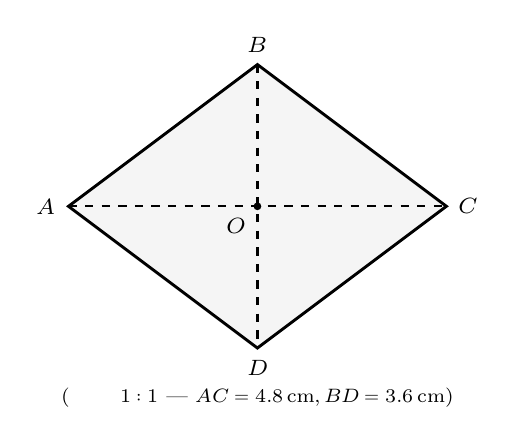
\begin{tikzpicture}[x=1cm, y=1cm, baseline={(0,1.40)}, every node/.style={font=\footnotesize, text=black}]
    \coordinate (A) at (-2.4,0);
    \coordinate (C) at (2.4,0);
    \coordinate (B) at (0,1.8);
    \coordinate (D) at (0,-1.8);
    \coordinate (O) at (0,0);
    \fill[gray!8] (A)--(B)--(C)--(D)--cycle;
    \draw[black, line width=1.05pt] (A)--(B)--(C)--(D)--cycle;
    \draw[black, line width=0.85pt, dashed] (A)--(C) (B)--(D);
    \fill[black] (O) circle (1.4pt) node[below left=1pt] {$O$};
    \node[left=1pt] at (A) {$A$};
    \node[above=1pt] at (B) {$B$};
    \node[right=1pt] at (C) {$C$};
    \node[below=1pt] at (D) {$D$};
    \node[anchor=north, font=\scriptsize] at (0,-2.18) {(ខ្នាតពិត $1:1$ — $AC=4.8\unit{cm}, BD=3.6\unit{cm}$)};
  \end{tikzpicture}
  &
  {\renewcommand{\arraystretch}{1.26}
  \begin{tabular}{|L{4.85cm}|L{6.55cm}|}
    \hline
    \rowcolor{subgray}\textbf{ធាតុដែលត្រូវវាស់} & \textbf{លទ្ធផលវាស់ និងការសង្កេត} \\
    \hline
    ជ្រុងទាំងបួន $AB, BC, CD, DA$ & $AB=\dotline{0.9cm}, BC=\dotline{0.9cm}, CD=\dotline{0.9cm}, DA=\dotline{0.9cm}\unit{cm}$ \\
    \hline
    \textbf{អន្ទាក់អង្កត់ទ្រូង៖} $AC$ ធៀបនឹង $BD$ & $AC=4.8\unit{cm}, BD=3.6\unit{cm}$ (\chk\ ស្មើ \chk\ មិនស្មើគ្នា) \\
    \hline
    មុំប្រសព្វត្រង់ផ្ចិត $\ang{AOB}$ & $\ang{AOB} = \dotline{1.3cm}^\circ \Rightarrow AC \dotline{0.9cm} BD$ \\
    \hline
    មុំពុះត្រង់កំពូល $\ang{BAO}$ និង $\ang{DAO}$ & $\ang{BAO}\approx\dotline{1.1cm}^\circ$, $\ang{DAO}\approx\dotline{1.1cm}^\circ$ (\chk\ ស្មើគ្នា) \\
    \hline
    ហេតុអ្វីខ្លែង $EFGH$ មានជ្រុង $EF \neq FG$? & ព្រោះត្រង់ផ្ចិត $O$ កំណាត់ $OE \neq \dotline{1.1cm}$ (មិនមែនប្រលេឡូក្រាម!) \\
    \hline
  \end{tabular}}
\end{tabular}

\vspace{5pt}
\textbf{សកម្មភាពទី២ — សម្រាយបញ្ជាក់តាមត្រីកោណប៉ុនគ្នាជុំវិញផ្ចិត $O$ (៦ នាទី)៖} គូស \textbf{[tracing]} លើជ្រុងរួម $AO$ រួចបំពេញ៖\par\vspace{3pt}
{\renewcommand{\arraystretch}{1.22}
\begin{tabular}{|L{9.15cm}|L{9.15cm}|}
  \hline
  \rowcolor{subgray}\textbf{ផ្នែក ក៖ ទ្រឹស្ដីបទទី២ និងទី៤ (ចតុកោណស្មើ $\Rightarrow AC\perp BD$ និងពុះមុំ)} & \textbf{ផ្នែក ខ៖ ទ្រឹស្ដីបទទី៣ (ប្រលេឡូក្រាមមាន $AC\perp BD \Rightarrow$ ចតុកោណស្មើ)} \\
  \hline
  \begin{center}
  \vspace{-2pt}
  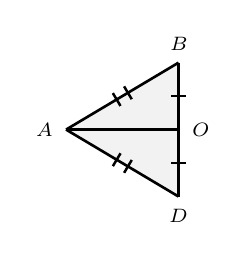
\begin{tikzpicture}[scale=0.68, every node/.style={font=\scriptsize}]
    \coordinate (A) at (-2.1,0); \coordinate (O) at (0,0);
    \coordinate (B) at (0,1.25); \coordinate (D) at (0,-1.25);
    \fill[gray!10] (A)--(B)--(D)--cycle;
    \draw[line width=0.95pt, tk2] (A)--(B);
    \draw[line width=0.95pt, tk2] (D)--(A);
    \draw[line width=0.95pt, tk1] (B)--(O);
    \draw[line width=0.95pt, tk1] (O)--(D);
    \draw[line width=1.05pt] (A)--(O);
    \node[left=1pt] at (A) {$A$}; \node[above=1pt] at (B) {$B$};
    \node[below=1pt] at (D) {$D$}; \node[right=1.5pt] at (O) {$O$};
  \end{tikzpicture}
  \vspace{-3pt}
  \end{center}
  ក្នុងចតុកោណស្មើ $ABCD$ ពិនិត្យ $\tri{ABO}$ និង $\tri{ADO}$៖\par
  ១. ជ្រុង $AB = \dotline{1.2cm}$ (ជ្រុងជាប់នៃចតុកោណស្មើ)\par
  ២. កំណាត់ $OB = \dotline{1.2cm}$ (អង្កត់ទ្រូងប្រលេឡូក្រាមកាត់ពាក់កណ្ដាលគ្នា)\par
  ៣. អង្កត់ $AO$ ជាជ្រុង \dotline{1.5cm} (\textbf{[tracing]})\par
  $\Rightarrow \tri{ABO} \cg \tri{ADO}$ តាមលក្ខណៈ (\dotline{1.4cm})\par
  $\bullet$ \textbf{វិបាកទី១៖} $\ang{AOB}=\ang{AOD}$ តែបូកគ្នា $=180^\circ \Rightarrow \ang{AOB}=\dotline{0.9cm}^\circ \Rightarrow AC\perp BD$\par
  $\bullet$ \textbf{វិបាកទី២៖} $\ang{BAO}=\ang{\dotline{1.1cm}} \Rightarrow AC$ ជាកន្លះបន្ទាត់ពុះមុំ $\ang{BAD}$ ។
  &
  \begin{center}
  \vspace{-2pt}
  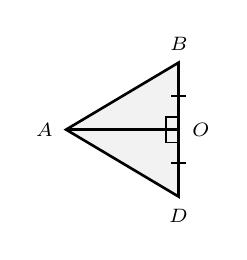
\begin{tikzpicture}[scale=0.68, every node/.style={font=\scriptsize}]
    \coordinate (A) at (-2.1,0); \coordinate (O) at (0,0);
    \coordinate (B) at (0,1.25); \coordinate (D) at (0,-1.25);
    \fill[gray!10] (A)--(B)--(D)--cycle;
    \draw[line width=0.95pt] (A)--(B)--(D)--cycle;
    \draw[line width=0.95pt, tk1] (B)--(O);
    \draw[line width=0.95pt, tk1] (O)--(D);
    \draw[line width=1.05pt] (A)--(O);
    \draw[line width=0.65pt] (-0.24,0)--(-0.24,0.24)--(0,0.24);
    \draw[line width=0.65pt] (-0.24,0)--(-0.24,-0.24)--(0,-0.24);
    \node[left=1pt] at (A) {$A$}; \node[above=1pt] at (B) {$B$};
    \node[below=1pt] at (D) {$D$}; \node[right=1.5pt] at (O) {$O$};
  \end{tikzpicture}
  \vspace{-3pt}
  \end{center}
  ក្នុងប្រលេឡូក្រាម $ABCD$ ដែលមាន $AC \perp BD$ ត្រង់ $O$៖\par
  ពិនិត្យ $\tri{ABO}$ និង $\tri{ADO}$ មាន៖\par
  ១. កំណាត់ $OB = \dotline{1.2cm}$ (ប្រលេឡូក្រាម)\par
  ២. មុំកែង $\ang{AOB} = \ang{\dotline{1.2cm}} = 90^\circ$ (សម្មតិកម្ម $AC\perp BD$)\par
  ៣. អង្កត់ $AO$ ជាជ្រុង \dotline{1.5cm}\par
  $\Rightarrow \tri{ABO} \cg \tri{ADO}$ តាមលក្ខណៈ (\dotline{1.4cm})\par
  $\bullet$ \textbf{វិបាក៖} ជ្រុងជាប់ $AB = \dotline{1.2cm} \Rightarrow ABCD$ ជា \dotline{2.4cm} ។ \\
  \hline
\end{tabular}}

\newpage

% ============================================================================
% ទំព័រទី២៖ E3 ធនាគារហេតុផល ①–⑤ + E4 លំហាត់គំរូ ២ + E5 ប្រតិបត្តិ & Exit Check + កិច្ចការផ្ទះ
% ============================================================================
\secbar{ផ្នែកទី៣ ៖ សង្ខេបលក្ខណៈចតុកោណស្មើ និងធនាគារហេតុផល \cnum{1}--\cnum{5} \enbf{(E3 -- Explain)}}{៦ នាទី}
\begin{tcolorbox}[enhanced, sharp corners, colback=white, colframe=black, boxrule=0.8pt, top=4pt, bottom=4pt, left=6pt, right=6pt]
  \cnum{1} \textbf{និយមន័យ និងទ្រឹស្ដីបទទី១៖} ចតុកោណស្មើ ជាប្រលេឡូក្រាមមានជ្រុងជាប់ពីរប៉ុនគ្នា $\Rightarrow$ ជ្រុងទាំងបួន \dotline{2.0cm} ($AB=BC=CD=DA$) ។\par\vspace{2pt}
  \cnum{2} \textbf{ទ្រឹស្ដីបទទី២៖} អង្កត់ទ្រូងទាំងពីរនៃចតុកោណស្មើ \dotline{2.0cm} ($AC \perp BD$ ត្រង់ចំណុចកណ្ដាល $O$) ។\par\vspace{2pt}
  \cnum{3} \textbf{ទ្រឹស្ដីបទទី៣ (សម្គាល់)៖} ប្រលេឡូក្រាមដែលមានអង្កត់ទ្រូង \dotline{1.8cm} ជាចតុកោណស្មើ (ឬចតុកោណមានជ្រុងទាំង ៤ ប៉ុនគ្នា) ។\par\vspace{2pt}
  \cnum{4} \textbf{ទ្រឹស្ដីបទទី៤៖} អង្កត់ទ្រូងនៃចតុកោណស្មើ ជាកន្លះបន្ទាត់ \dotline{2.2cm} នៃមុំឈម និងជាអ័ក្សឆ្លុះ ។\par\vspace{2pt}
  \cnum{5} \textbf{មុំបំពេញកែង៖} ក្នុងត្រីកោណកែង $\tri{OCD}$ ($\ang{DOC}=90^\circ$) គេបាន $\ang{ODC} + \ang{OCD} = \dotline{1.1cm}^\circ$ ។
\end{tcolorbox}

% --- E4 Elaborate ---
\secbar{ផ្នែកទី៤ ៖ លំហាត់គំរូអនុវត្ត \enbf{[tracing]} និងធនាគារហេតុផល \cnum{1}--\cnum{5} \enbf{(E4 -- Elaborate)}}{១០ នាទី}
{\renewcommand{\arraystretch}{1.24}
\begin{tabular}{|L{9.15cm}|L{9.15cm}|}
  \hline
  \rowcolor{subgray}\textbf{គំរូទី១ (លំហាត់គំរូ ទំ.១៧៨--១៧៩ — ចតុកោណស្មើ $AOBI$)} & \textbf{គំរូទី២ (លំហាត់ទី១២ ទំ.១៨៦ — ភ្ជាប់តាមត្រីកោណសមបាត $\tri{CDE}$)} \\
  \hline
  គេមានចតុកោណកែង $ABCD$ មានអង្កត់ទ្រូងកាត់គ្នាត្រង់ $O$ ។ គេសង់ប្រលេឡូក្រាម $AOBI$ ។ បង្ហាញថា $AOBI$ ជាចតុកោណស្មើ ។\par
  \begin{center}
  \vspace{-1pt}
  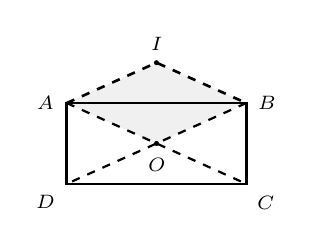
\begin{tikzpicture}[scale=0.76, every node/.style={font=\scriptsize}]
    \coordinate (D) at (0,0); \coordinate (C) at (3.00,0);
    \coordinate (A) at (0,1.35); \coordinate (B) at (3.00,1.35);
    \coordinate (O) at (1.50,0.675); \coordinate (I) at (1.50,2.025);
    \fill[gray!12] (A)--(I)--(B)--(O)--cycle;
    \draw[line width=0.95pt] (A)--(B)--(C)--(D)--cycle;
    \draw[line width=0.8pt, dashed] (A)--(C) (B)--(D);
    \draw[line width=0.95pt, dashed] (A)--(I)--(B);
    \fill (O) circle (1.2pt) node[below=1.5pt] {$O$};
    \fill (I) circle (1.2pt) node[above=1pt] {$I$};
    \node[left=1pt] at (A) {$A$}; \node[right=1pt] at (B) {$B$};
    \node[below right=1pt] at (C) {$C$}; \node[below left=1pt] at (D) {$D$};
  \end{tikzpicture}
  \vspace{-1pt}
  \end{center}
  $\bullet$ ក្នុងចតុកោណកែង $ABCD$៖ កំណាត់អង្កត់ទ្រូង $AO = \dotline{1.0cm}$\par
  $\bullet$ ក្នុងប្រលេឡូក្រាម $AOBI$៖ ជ្រុងឈម $AI = \dotline{1.0cm}$\par
  $\bullet$ នាំឱ្យជ្រុងជាប់ $AO = \dotline{1.0cm}$\par
  $\bullet$ ដូច្នេះប្រលេឡូក្រាម $AOBI$ ជា \dotline{2.3cm} (តាម \cnum{1}) ។
  &
  ក្នុងប្រលេឡូក្រាម $ABCD$ គេមាន $AD=CE$ និង $\ang{CDE}=\ang{CED}$ ($E$ ស្ថិតលើបន្ទាត់ $BC$) ។ បង្ហាញថា $ABCD$ ជាចតុកោណស្មើ ។\par
  \begin{center}
  \vspace{-1pt}
  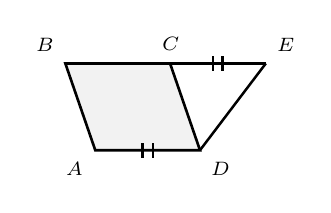
\begin{tikzpicture}[scale=0.76, every node/.style={font=\scriptsize}]
    \coordinate (B) at (0,1.45); \coordinate (C) at (1.75,1.45); \coordinate (E) at (3.35,1.45);
    \coordinate (A) at (0.50,0); \coordinate (D) at (2.25,0);
    \fill[gray!10] (A)--(B)--(C)--(D)--cycle;
    \draw[line width=0.95pt] (A)--(B)--(C)--(D)--cycle;
    \draw[line width=0.9pt, tk2] (A)--(D);
    \draw[line width=0.9pt, tk2] (C)--(E);
    \draw[line width=0.9pt] (D)--(E);
    \node[below left=1pt] at (A) {$A$}; \node[above left=1pt] at (B) {$B$};
    \node[above=1pt] at (C) {$C$}; \node[below right=1pt] at (D) {$D$};
    \node[above right=1pt] at (E) {$E$};
  \end{tikzpicture}
  \vspace{-1pt}
  \end{center}
  $\bullet$ ក្នុង $\tri{CDE}$៖ ដោយ $\ang{CDE}=\ang{CED}$ នោះ $CD = \dotline{1.0cm}$\par
  $\bullet$ តែតាមសម្មតិកម្ម $AD = CE$ នាំឱ្យ $AD = \dotline{1.0cm}$\par
  $\bullet$ ប្រលេឡូក្រាម $ABCD$ មានជ្រុងជាប់ $AD$ និង $CD$ \dotline{1.6cm}\par
  $\bullet$ ដូច្នេះ $ABCD$ ជា \dotline{2.3cm} (តាម \cnum{1}) ។ \\
  \hline
\end{tabular}}\par\vspace{3pt}
$\bullet$ \textbf{ឆ្លុះបញ្ចាំង (\en{EIA})៖} ផ្លូវទាំង ២ ដើម្បីបង្ហាញថាប្រលេឡូក្រាមជាចតុកោណស្មើ គឺ (១) \dotline{3.6cm} ឬ (២) \dotline{3.6cm} ។

% --- E5 Evaluate ---
\secbar{ផ្នែកទី៥ ៖ លំហាត់ប្រតិបត្តិ ផ្ទៀងផ្ទាត់ជាដៃគូ និង \enbf{Exit Check (E5 -- Evaluate)}}{១០ នាទី}
\textbf{ក. លំហាត់ប្រតិបត្តិ (ទំព័រ ១៧៩)៖} គណនារង្វាស់មុំ $\ang{DAB}, \ang{BDC}$ និង $\ang{ABC}$ នៃចតុកោណស្មើ $ABCD$ ដែលមាន $AB=BC=CD=DA=BD$ ។\par\vspace{3pt}
\begin{tabular}{@{}L{13.15cm} C{5.65cm}@{}}
  ១. ប្រភេទនៃត្រីកោណ $\tri{ABD}$ និង $\tri{CBD}$៖ ជាត្រីកោណ \dotline{3.5cm} $\Rightarrow \ang{DAB} = \dotline{1.1cm}^\circ$\par\vspace{5pt}
  ២. រង្វាស់មុំ $\ang{BDC} = \dotline{1.2cm}^\circ$ និងមុំធំ $\ang{ABC} = \ang{ABD}+\ang{CBD} = \dotline{2.2cm}^\circ$\par\vspace{5pt}
  ៣. \textbf{បិទបញ្ហាខ្លែង E1៖} សិស្ស ក ខុស ព្រោះក្នុងរូបខ្លែង $OE \neq OG$ (មិនមែនជា \dotline{2.6cm})
  &
  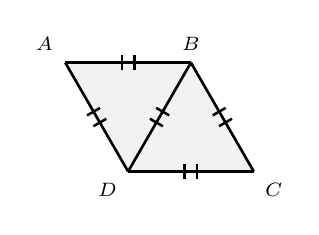
\begin{tikzpicture}[scale=0.84, baseline={(0,1.40)}, every node/.style={font=\scriptsize}]
    \coordinate (D) at (0.95,0); \coordinate (C) at (2.85,0);
    \coordinate (A) at (0,1.645); \coordinate (B) at (1.90,1.645);
    \fill[gray!10] (A)--(B)--(C)--(D)--cycle;
    \draw[line width=0.95pt, tk2] (A)--(B);
    \draw[line width=0.95pt, tk2] (B)--(C);
    \draw[line width=0.95pt, tk2] (C)--(D);
    \draw[line width=0.95pt, tk2] (D)--(A);
    \draw[line width=0.95pt, tk2] (B)--(D);
    \node[above left=1pt] at (A) {$A$}; \node[above=1pt] at (B) {$B$};
    \node[below right=1pt] at (C) {$C$}; \node[below left=1pt] at (D) {$D$};
  \end{tikzpicture}
\end{tabular}

\vspace{5pt}
\begin{tcolorbox}[enhanced, sharp corners, colback=panelgray, colframe=black, boxrule=0.8pt, top=4pt, bottom=4pt, left=6pt, right=6pt]
  \textbf{ខ. សំណួរត្រួតពិនិត្យរហ័ស (\en{Exit Check} — គូសរង្វង់ចម្លើយត្រឹមត្រូវតែ ១)៖}\par
  ក្នុងចតុកោណស្មើ $ABCD$ (ផ្ចិត $O$) បើ $\ang{BAC} = 35^\circ$ តើរង្វាស់មុំពេញ $\ang{BAD}$ និងមុំ $\ang{ABD}$ ស្មើប៉ុន្មាន?\par\vspace{2pt}
  \hspace*{0.2cm}\textbf{A.} $35^\circ$ និង $55^\circ$ \hspace{1.1cm} \textbf{B.} $70^\circ$ និង $55^\circ$ \hspace{1.1cm} \textbf{C.} $70^\circ$ និង $35^\circ$ \hspace{1.1cm} \textbf{D.} $70^\circ$ និង $110^\circ$
\end{tcolorbox}

% --- Step 5 Homework ---
\secbar{ផ្នែកទី៦ ៖ កិច្ចការផ្ទះ និងបណ្ដាំផ្ញើ \enbf{(}ទំព័រ ១៨៥--១៨៦\enbf{)}}{ធ្វើក្នុងសៀវភៅកិច្ចការផ្ទះ}
$\bullet$ \textbf{លំហាត់ទី១ (ទំ.១៨៥)៖} សង់ចតុកោណស្មើ $ABCD$ ដោយស្គាល់ប្រវែងអង្កត់ទ្រូង $AC = 5\unit{cm}$ និង $BD = 8\unit{cm}$ (គូសអង្កត់ទ្រូងកែងគ្នាត្រង់ចំណុចកណ្ដាលរៀងៗខ្លួន៖ $OA=OC=2.5\unit{cm}, OB=OD=4\unit{cm}$) ។\par\vspace{2.5pt}
$\bullet$ \textbf{លំហាត់ទី១៣ និងទី១៤ (ទំ.១៨៦)៖} ក្នុងចតុកោណស្មើ $ABCD$ (ផ្ចិត $O$)៖ (ក) បើគូសកម្ពស់ $BE\perp AD$ និង $DF\perp BC$ បង្ហាញថា $BE=DF$; (ខ) បង្ហាញថា $\ang{ODC}+\ang{OCD}=90^\circ$ ហើយអានជាមុន \textbf{២.៤ លក្ខណៈការេ និងទ្រឹស្ដីបទចំណុចកណ្ដាល} (ទំ.១៧៩--១៨១) ។

\end{document}
